\documentclass[12pt]{report}
\usepackage{pgfplots}

\pgfplotsset{
	curve plot style/.style={
		xlabel={N - Number of top database candidates},
		xmin=0, xmax=25,
		xtick={0,5,10,15,20,25},
		ytick={45,50,55,60,65,70,75,80,85,90,95,100},
		legend pos=south east,
		ymajorgrids=true,     xmajorgrids=true,
		grid style=dashed,
		ylabel={Recall@N (\%)},
		ylabel style={yshift=-.3cm},
		width=8.5cm,
		height=10cm,
	},
}


\usepackage[margin=0.5in]{geometry}
\usepackage[utf8]{inputenc}
\usepackage{epsfig} %
\usepackage{ tipa }
\usepackage{ textcomp }
\usepackage{float}
\usepackage{ dsfont }
\usepackage{multirow}
\usepackage{ltablex}
\usepackage{siunitx}
\usepackage{subfloat}
\usepackage{pdfpages}
\usepackage{moreverb,url}
\usepackage{cite}
\usepackage{makecell}
%\SIsetup{table-format=-2.0, table-number-alignment=center}
%\usepackage[colorlinks,bookmarksopen,bookmarksnumbered,citecolor=red,urlcolor=red]{hyperref}
\usepackage[colorlinks=true,linkcolor=black,citecolor=blue,urlcolor=blue,]{hyperref}
\usepackage[ruled,vlined,noresetcount]{algorithm2e}
\usepackage[noend]{algpseudocode}
\usepackage[
font=footnotesize %
]{subfig}


\usepackage{amsmath,amssymb,amsfonts}
\usepackage{graphicx}
\usepackage{textcomp}
\usepackage{xcolor}
\usepackage{bm}
\newcommand*{\rom}[1]{\expandafter\@slowromancap\romannumeral #1@}
\SetKwFunction{KwFn}{Fn}
%\SetKwProg{Fn}{Function}{}{}
\linespread{1.5}

\setlength{\topmargin}{-0.5cm}
\setlength{\textheight}{23.5cm}
\setlength{\oddsidemargin}{1.5cm}
\setlength{\evensidemargin}{0cm}
\setlength{\textwidth}{14.4cm}
\setlength{\headsep}{0in}
\setlength{\parskip}{.15in}
\setlength{\parindent}{0in}

\usepackage{setspace} %

\usepackage{nomencl}
\makenomenclature
\renewcommand{\nomname}{ABBREVIATIONS}

\definecolor{Mycolor2}{HTML}{1560BD}
\newcommand{\colorit}[1]{{\color{Mycolor2}{#1}}}
\usepackage{xcolor}
\definecolor{mediumBlue}{rgb}{0.15,0.15,0.75}
\definecolor{darkBlue}{rgb}{0,0,0.5}


\usepackage{float}
\usepackage{tikz,xcolor}
\usepackage{xcolor}
\usepackage{tcolorbox}

\usepackage{bibentry}
\usepackage[numbers,sort&compress,sectionbib]{natbib}
%\usepackage{chapterbib}
\DeclareMathOperator{\tr}{Tr}

%\bibliographystyle{ieeetr}



\newcommand{\thesisWriter}{XXX}
\newcommand{\ThesisTitle}{\Large\bf Thesis title goes here}

\begin{document}

\pagenumbering{Roman}

\addcontentsline{toc}{chapter}{Title Page}

%\thispagestyle{empty}
\null\vspace{0.5in}
\begin{center}
	{\huge \bf \thesisWriter}
	\vspace{2.5cm}
	
	{\Large by}
	\vspace{0.5cm}
	
	{\Large\bf \ThesisTitle{}}\normalsize
	\vspace{2.5cm}
	
	A Thesis Submitted to \\
	The Hong Kong University of Science and Technology \\
	in Partial Fulfillment of the Requirements for \\
	the Degree of Doctor of Philosophy \\
	in the Department of Physics
	\vspace{1.5cm}
	
	March 2024, Hong Kong
\end{center}

\newpage

%\pagenumbering{Roman}
\addcontentsline{toc}{chapter}{Authorization Page}
\begin{center}{\Large\bf Authorization}\normalsize
\end{center}
\vspace{0.5cm}

I hereby declare that I am the sole author of the thesis.

\vspace{0.5cm}

I authorize the Hong Kong University of Science and Technology to lend this thesis
to other institutions or individuals for the purpose of scholarly research.

\vspace{0.5cm}

I further authorize the Hong Kong University of Science and Technology to
reproduce the thesis by photocopying or by other means, in total or in
part, at the request of other institutions or individuals for the
purpose of scholarly research.

\vspace{0.3cm}

\begin{figure}[h]
	\centering
	
\includegraphics[scale=.30]{includes/sign.png}
\end{figure}
\begin{center}
	\vspace*{-1.9cm}
	\line(1,0){180}
	\smallskip
	
	\thesisWriter{}
	
	March 2024, Hong Kong
\end{center}

\newpage

\addcontentsline{toc}{chapter}{Signature Page}
\null\vspace{0.4cm}
\begin{center}
	{\Large\bf \ThesisTitle{}}
	\vspace{1.5cm}
	
	{by}\smallskip
	
	{\thesisWriter{}}\normalsize
	
	\vspace{1cm}
	
	This is to certify that I have examined the above PhD thesis and have found that it is complete and satisfactory in all respects, and that any and all revisions required by the thesis examination committee have been made.
	
	\vspace{1.5cm}
	
	\line(1,0){230} 
	
	Professor XoX (Physics), Thesis Supervisor
	
	\vspace{1.5cm}
	
	\line(1,0){230} 
	
	Professor X-X (Physics), Head of the Physics Department
	
	\vspace{2cm}
	Department of Physics \\
	The Hong Kong University of Science and Technology \\
	March 2024, Hong Kong
\end{center}




\newpage

\addcontentsline{toc}{chapter}{Acknowledgments}
\begin{center}{\Large\bf Acknowledgment}\normalsize
\end{center}
\vspace{0.5cm}

{.
	32\it Acknowledgment goes here}

 
\vfill

\newpage

\addcontentsline{toc}{chapter}{Table of Contents}

\begin{spacing}{0.25}
   {\footnotesize \tableofcontents}
\end{spacing}

\newpage
\addcontentsline{toc}{chapter}{List of Figures}
\listoffigures

\newpage
\addcontentsline{toc}{chapter}{List of Tables}
\listoftables


\newpage


\newpage
\addcontentsline{toc}{chapter}{Abbreviations}
\printnomenclature[1in]

\newpage
\pagenumbering{arabic}



\addcontentsline{toc}{chapter}{Abstract}
\begin{center}
{\Large\bf Simulation Investigation of Active and Driven Flows in Achiral and Chiral Nematics}
\vspace{0.5cm}

{\large \bf \thesisWriter{}}\normalsize

\medskip

Department of Physics\\ The Hong Kong University of Science and Technology

\end{center}
\vspace{1.5cm}
\centerline{{\bf \large Abstract}}
\vspace{1.5cm}

{\it Abstract goes here.}


\chapter{Introduction}\label{ch1-intro}

\section{`First part'}

\section{`Second part'}

\section{`Third part'}


\section{Thesis Contributions}


\chapter{Theory and Methods}
\label{sec-theory}


\section{`1st section'}
\label{chapter_2_fo_ldg}

\subsection{'1st Subsection'}
\label{FO_theory}



\subsection{`2nd Subsection'}
\label{LdG_theory}

	


\chapter{First Project}
\label{sec-crystals}


\begin{figure}[!h]
	\centering
	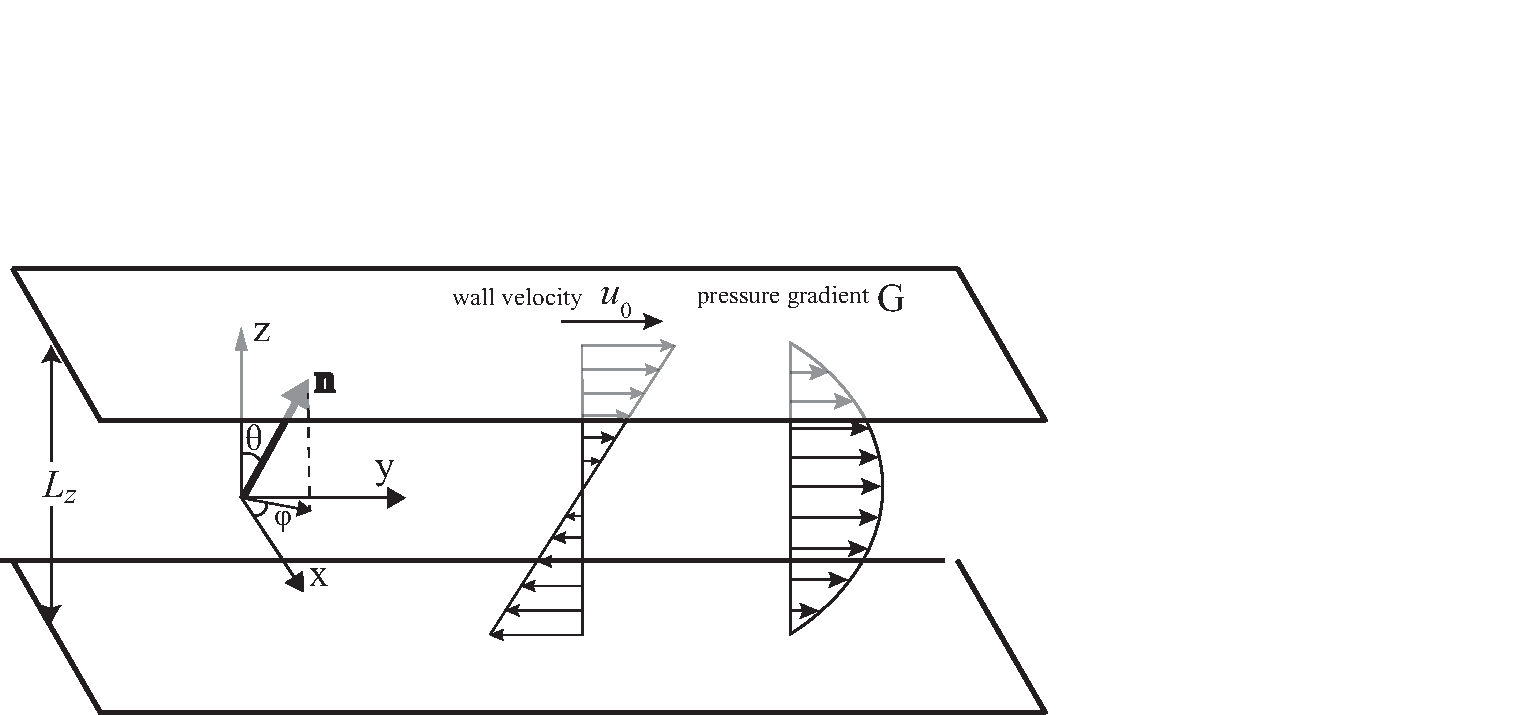
\includegraphics[width=1.0\linewidth]{images/Result1/figure1_setup.pdf}
	\caption{ {\bf Simulation setup.} Two walls are in $z$-direction separated by a distance of \emph{$L_z$}. Easy axis is in the $y$-direction. Couette flow is imposed by moving top and bottom wall in $y$-direction with speed $u_0$ and $-u_0$, respectively. Poiseuille flow is imposed by applying a pressure gradient \emph{$G$} along $y$-direction. Director field ${\bf n}$ is represented by a polar angle $\theta$ and an azimuthal angle $\phi$.}
	\label{fig2:setup}
\end{figure}


In this study, we conduct all the simulation in this flat channel Fig.~\ref{fig2:setup}. 


\section{Results-1st section}


\newpage
\section{Results-2nd section}

\newpage
\section{Conclusion}

-{\it Your conclusion of 1st project goes here}


\newpage

\section{Appendix}
\label{sec.appen}

\subsection{1st part of Appendix}
\label{appen_Leslie}
\chapter{2nd Project}
\label{sec-natcomm}

-{\it Your table goes as following example}

\vspace{0.2cm}
\begin{table}[h!]
	\centering
		\caption{{Handedness of the periodic double-twist configuration, obtained in 21 independent simulations.}}
   \begin{tabular}{|c|c|c|}
   \hline
								  &{\makecell[c]{left-handed twist \\ in $x$-direction }} & {\makecell[c]{right-handed twist \\ in $x$-direction}} \\ \hline
   {\makecell[c]{left-handed twist \\ in $z$-direction}}  & 10             & 0                  \\ \hline
   {\makecell[c]{right-handed twist \\ in $z$-direction}} & 0             & 11                  \\ \hline
   \end{tabular}
   \label{table1}
\end{table}

\chapter{3rd Project}
\label{sec-prl}

-{\it The 3rd Project goes here}


\chapter{Conclusion and Future Work}
\label{sec-conclusion}
-{\it A biref summary goes here}

\section{Conculsion}



\subsection{1st Project}
In the Chapter.~\ref{sec-crystals}

\subsection{2nd Project}


\subsection{3rd Project}


\section{Future Work and Challenges}




\newpage
\renewcommand*{\bibname}{\section*{\refname}}%
%\addcontentsline{toc}{chapter}{References}
\addcontentsline{toc}{chapter}{References}
\bibliographystyle{ieeetr}
\bibliography{thesis}	

\newpage
\renewcommand*{\bibname}{\section*{\refname}}%
\addcontentsline{toc}{chapter}{List of Publications}
%\null\vspace{0.5in}
\begin{center}
	{\LARGE\bf List of Publications}
\end{center}

{\Large{\bf{Jounrnal}}}

$\bullet$	{\bf Wang, W.}, Ren, H. and Zhang, R. (2024). Symmetry breaking of self-propelled topological defects in thin-film active chiral nematics, \emph{Physical Review Letters}, vol. 132(3). doi:10.1103/physrevlett.132.038301. 

\null\vspace{0.5in}
{\Large{\bf{Conference}}}

$\bullet$   (Oral) {\bf{Wang, W.}}, Ren, H., Zhang, R.. Symmetry breaking of self-propelled topological defects in thin-film active chiral nematics. \emph{American Physical Society March Meeting}, Las Vegas, 2023.



\end{document}
